\documentclass[master.tex]{subfiles}
\begin{document}
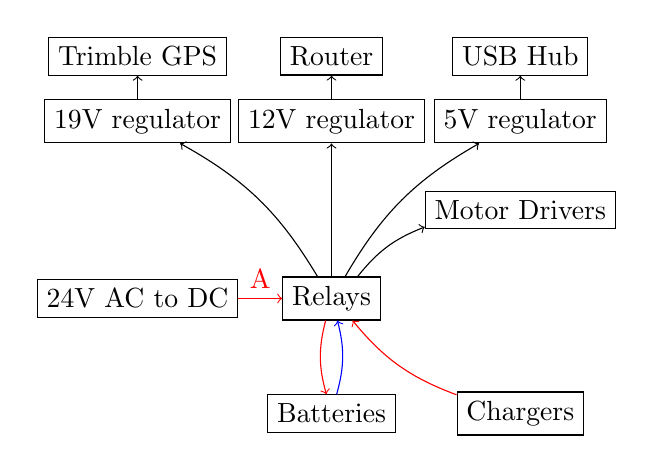
\begin{tikzpicture}[bend angle=15]
  \matrix [column sep=0mm,row sep=3mm] {
    \node[draw,shape=rectangle] (GPS) {Trimble GPS}; 
    & \node[draw,shape=rectangle] (Router) {Router}; 
    & \node[draw,shape=rectangle] (usb)  {USB Hub}; \\
    \node[draw,shape=rectangle] (19reg) {19V regulator}; 
    & \node[draw,shape=rectangle] (12reg) {12V regulator}; 
    & \node[draw,shape=rectangle] (5reg)  {5V regulator}; \\
    \\
    & & \node[draw,shape=rectangle] (motors) {Motor Drivers}; \\
    \\
    \node[draw,shape=rectangle] (24Vsource) {24V AC to DC};
    & \node[draw,shape=rectangle] (relays) {Relays}; \\
    \\
    \\
    & \node[draw,shape=rectangle] (batteries) {Batteries}; 
    & \node[draw,shape=rectangle] (chargers) {Chargers}; \\
  };
  \draw[->] (19reg)     edge (GPS);
  \draw[->] (12reg)     edge (Router);
  \draw[->] (5reg)      edge (usb);
  \draw[->] (relays)    edge [bend right] (19reg);
  \draw[->] (relays)    edge (12reg);
  \draw[->] (relays)    edge [bend left] (5reg) ;
  \draw[->] (relays)    edge [bend left] (motors) ;
  \draw[->,red] (24Vsource) edge node[above] {A}  (relays) ;
  \draw[<-,red] (batteries) edge [bend left](relays) ;
  \draw[->,blue] (batteries) edge [bend right] (relays) ;
  \draw[->,red] (chargers)  edge [bend left](relays) ;
\end{tikzpicture}
\end{document}
